\documentclass[10pt]{beamer}
\usepackage[utf8]{inputenc}
\usepackage[brazilian]{babel}
\usepackage[T1]{fontenc}
\usepackage{amsthm,amsfonts}
\usepackage[normalem] {ulem}
\usepackage{graphicx}
%\usepackage{epsfig}
%\usepackage{setspace}
%\usepackage{makeidx}
\usepackage{empheq,amsmath,amsfonts, amssymb,amsthm}
\usepackage{amsmath,amssymb}
\usepackage{amsmath}
\usepackage{amsfonts}
%\usepackage{color}
%\usepackage{times}
\usepackage{amssymb,indentfirst}
\usepackage{amscd}
%\usepackage{tikz,pgf}
%\usepackage{wrapfig}
%\usepackage{anysize}
%\usepackage{makeidx}
\usepackage{pgf,tikz}
\usetheme{Antibes}
\usepackage[colorlinks, linkcolor = blue, hyperindex]{hyperref}

\theoremstyle{definition}
\newtheorem{defi}{Definição}
\newtheorem{exem}{Exemplo}
\newtheorem{res}{Resolução}
\newtheorem{cor}{Corolário}
\newtheorem{teo}{Teorema}
\newtheorem{prop}{Proposição}

\title[Curva de Bézier e Casteljau]{Curva de Casteljau e Bézier}
\author[Oziel Ramos]{Oziel Ramos de Lima Junior  \\ Modelagem Geométrica}
\institute[UFAM \and ICE \and DM]{UNIVERSIDADE FEDERAL DO AMAZONAS \\ INSTITUTO DE CIÊNCIAS EXATAS E DA TERRA \\DEPARTAMENTO DE MATEMÁTICA \\ CURSO DE VERÃO}
\date{2023}
\logo{
\includegraphics[width=0.1\linewidth]{Ufam}}
\begin{document}
\maketitle

\begin{frame}{Sumário}
    \tableofcontents
\end{frame}

\section{Introdução}
\begin{frame}{Introdução}
    Este trabalho tem o objetivo de realizar a implementação da curva de casteljau e bézier, utilizando linguagem de programação python $3.10.9$. Foram utilizados as bibliotecas:\begin{itemize}
        \item Matplotlib $3.6.3$
        \item Numpy $1.24.1$
    \end{itemize}

    Todos os códigos utilizados e histórico de construção deles está contido no link do 
 \href{https://github.com/oziieljuniior/GM}{GitHub}  
\end{frame}

\begin{frame}
    \href{https://github.com/oziieljuniior/GM}{GitHub}
    \begin{center}
        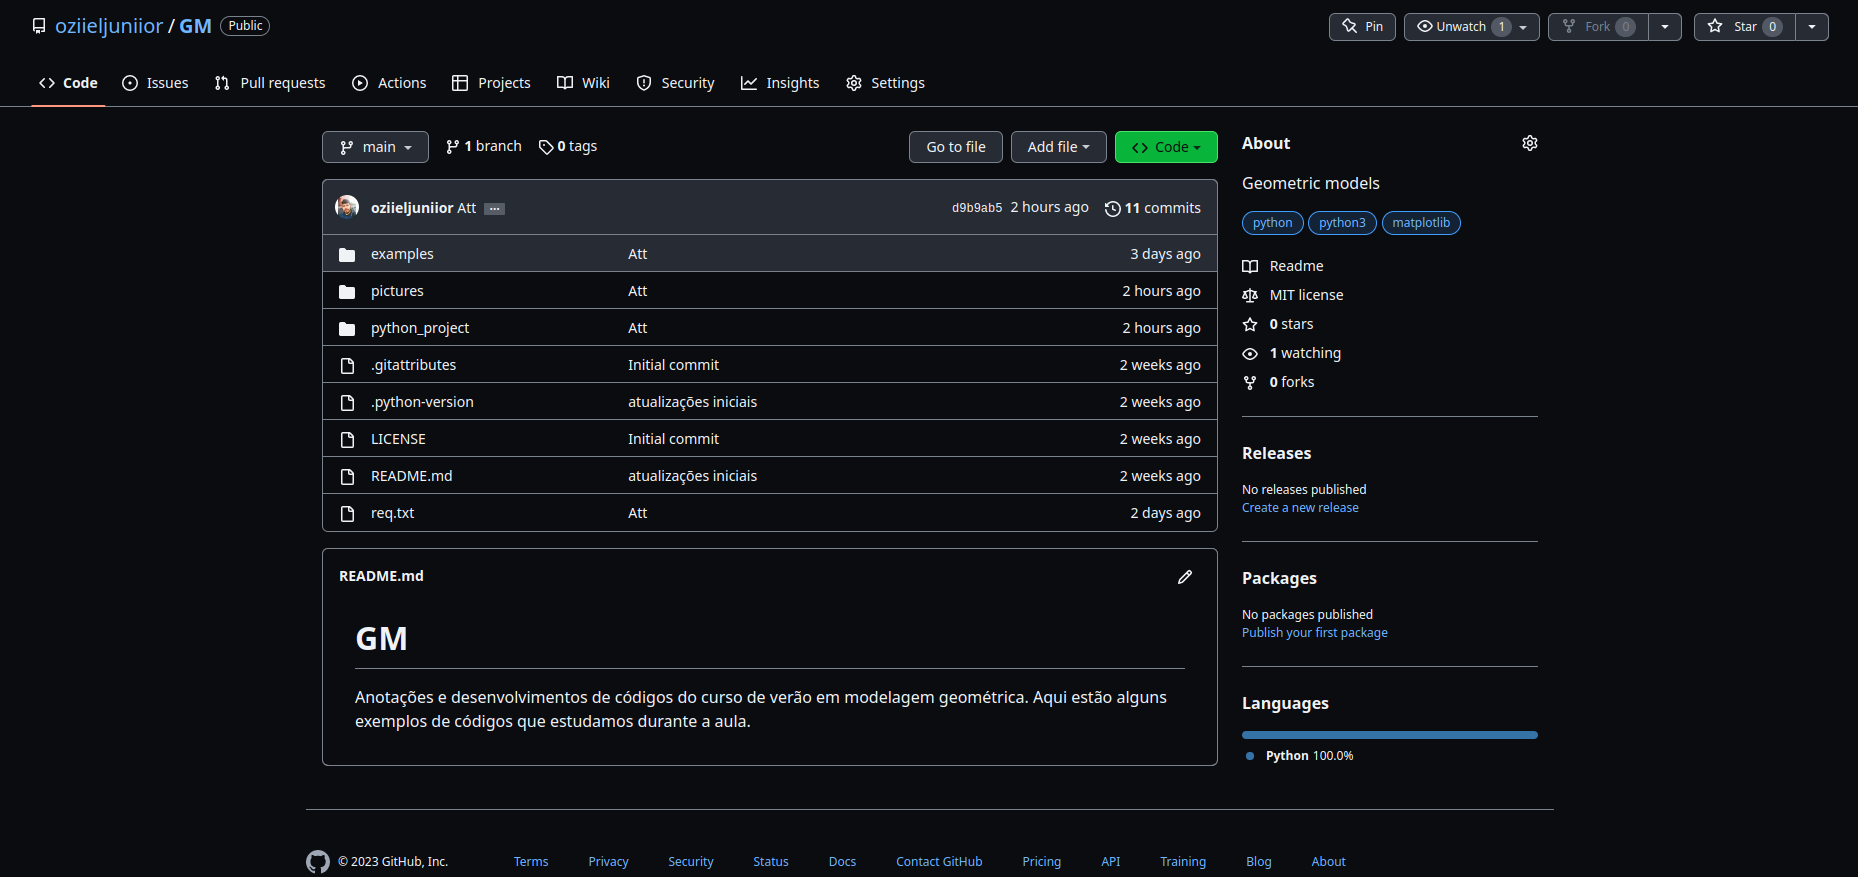
\includegraphics[width = 1 \linewidth]{Page_Github.png}
    \end{center}
\end{frame}

\section{Curva de Casteljau e Bézier}
\subsection{Teste}
\begin{frame}{Teste da Curva}
    \begin{center}
        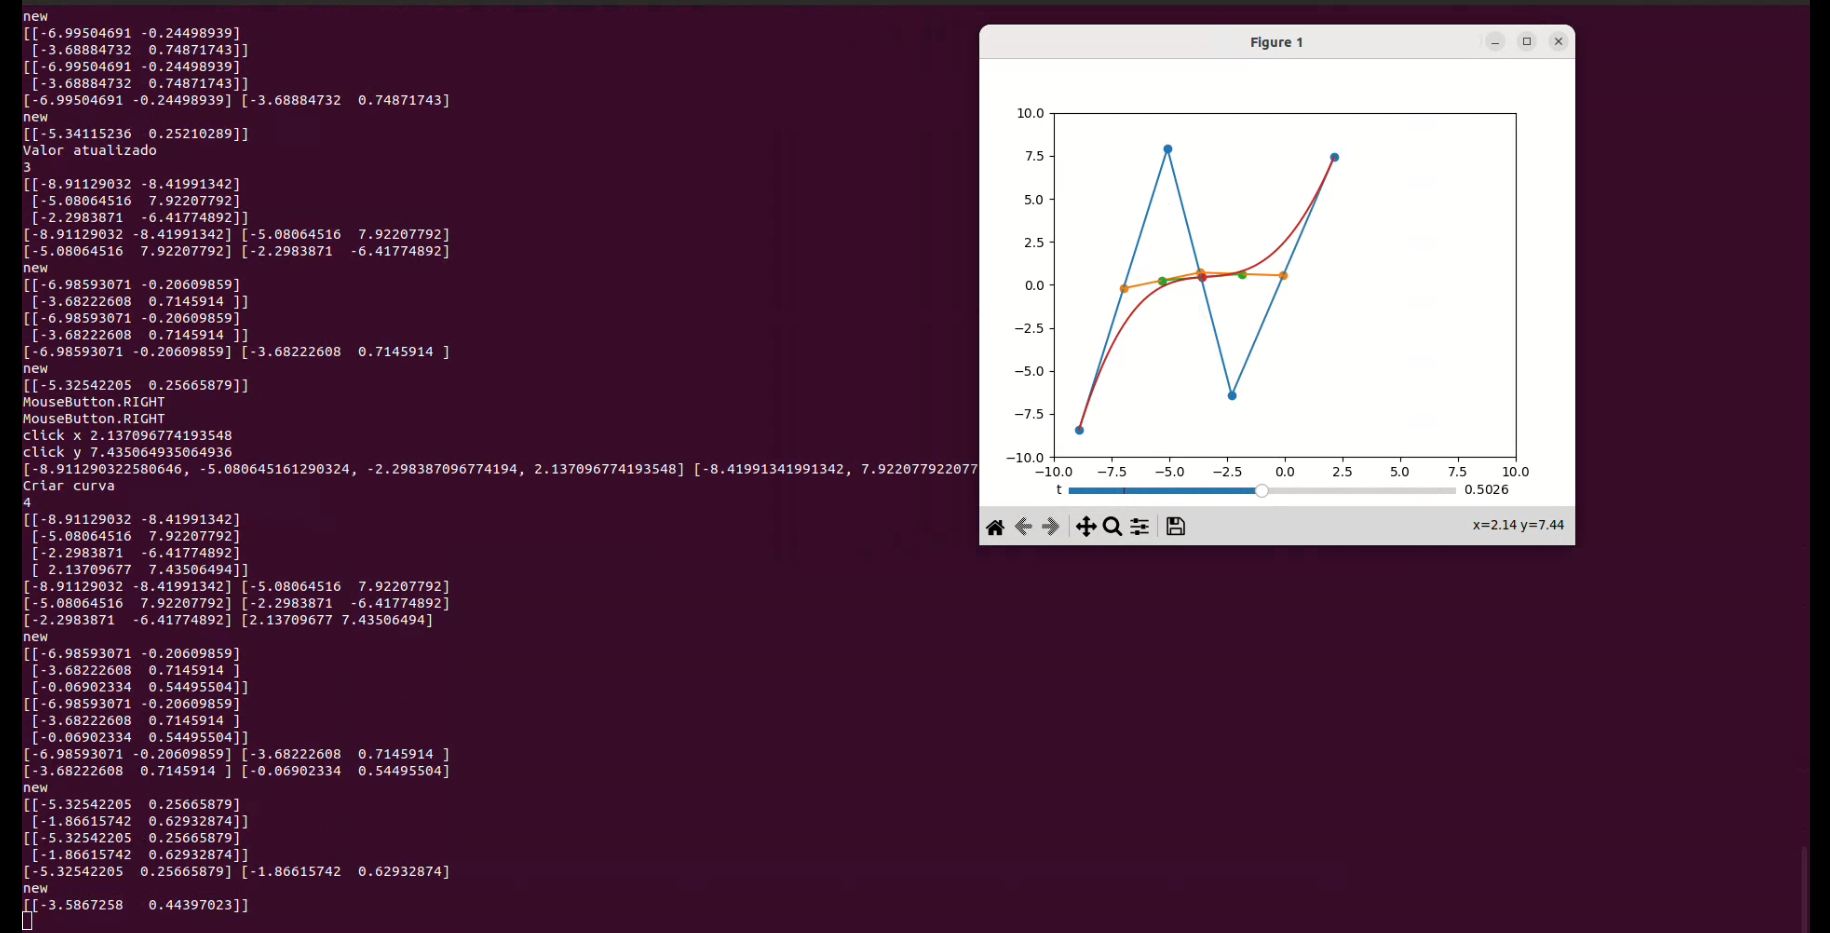
\includegraphics[width = 1 \linewidth]{teste1.png}
    \end{center}
\end{frame}
\subsection{Elaboração do Código}
\subsubsection{Bibliotecas Padrões}
\begin{frame}{Bibliotecas Padrões}
    
    \only<1> {É possível encontrar na web várias exemplos de códigos da curva de bézier
    \begin{center}
        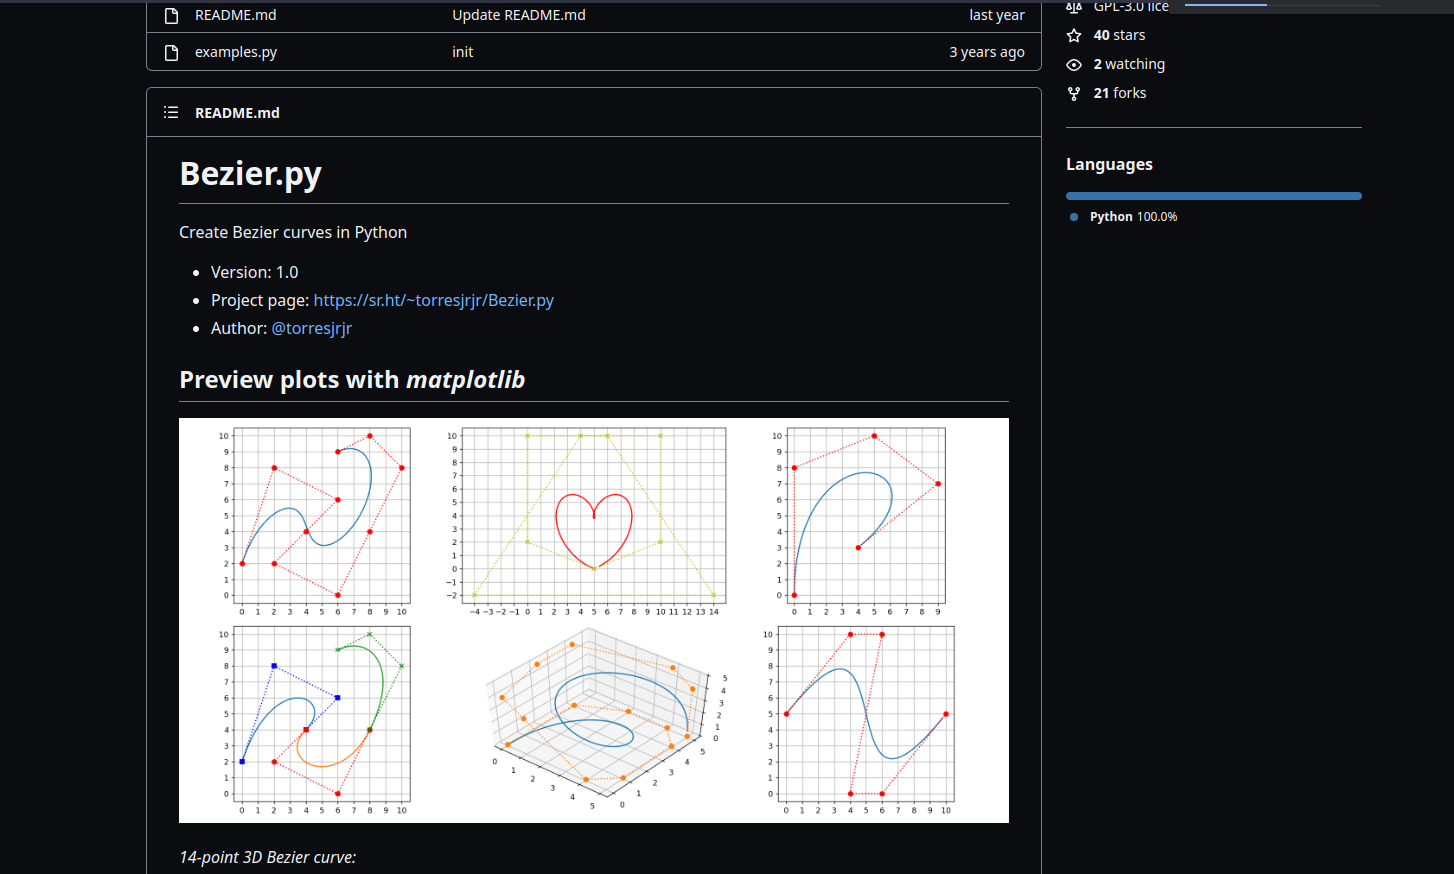
\includegraphics[width = 0.9 \linewidth]{bezier_code1.png}
    \end{center}}

    \only<2> {Tal como exercícios de faculdade 
    \begin{center}
        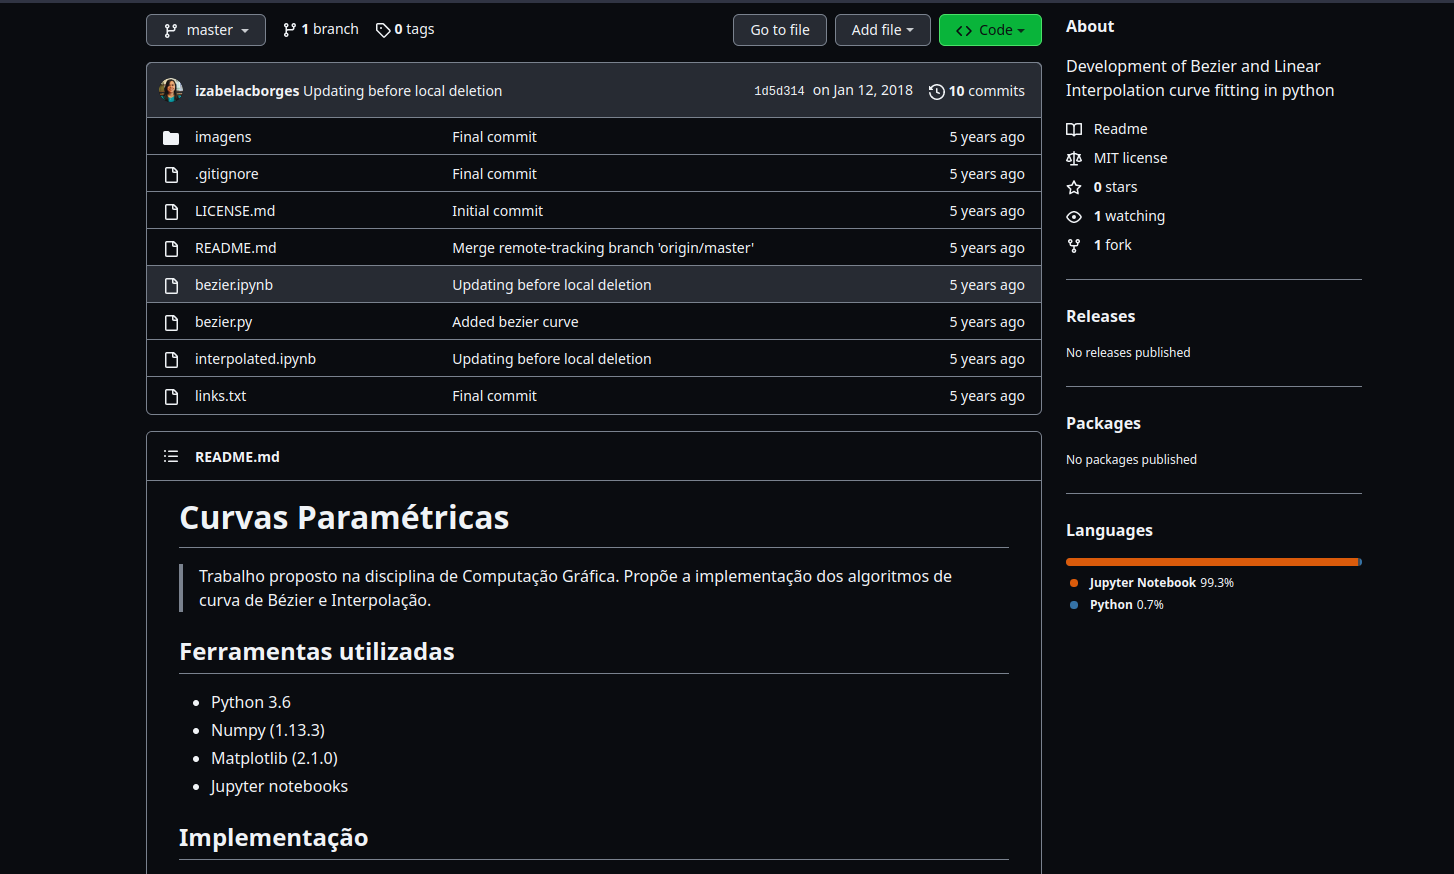
\includegraphics[width = 0.9 \linewidth]{bezier_code2.png}
    \end{center}
    }
    \only<3,4>{Existe um comando para a curva de bézier na biblioteca matplotlib. Na sua documentação, é possível ver que o algoritmo elaborado utiliza o algoritmo de Casteljau
    \begin{center}
        \only<3>{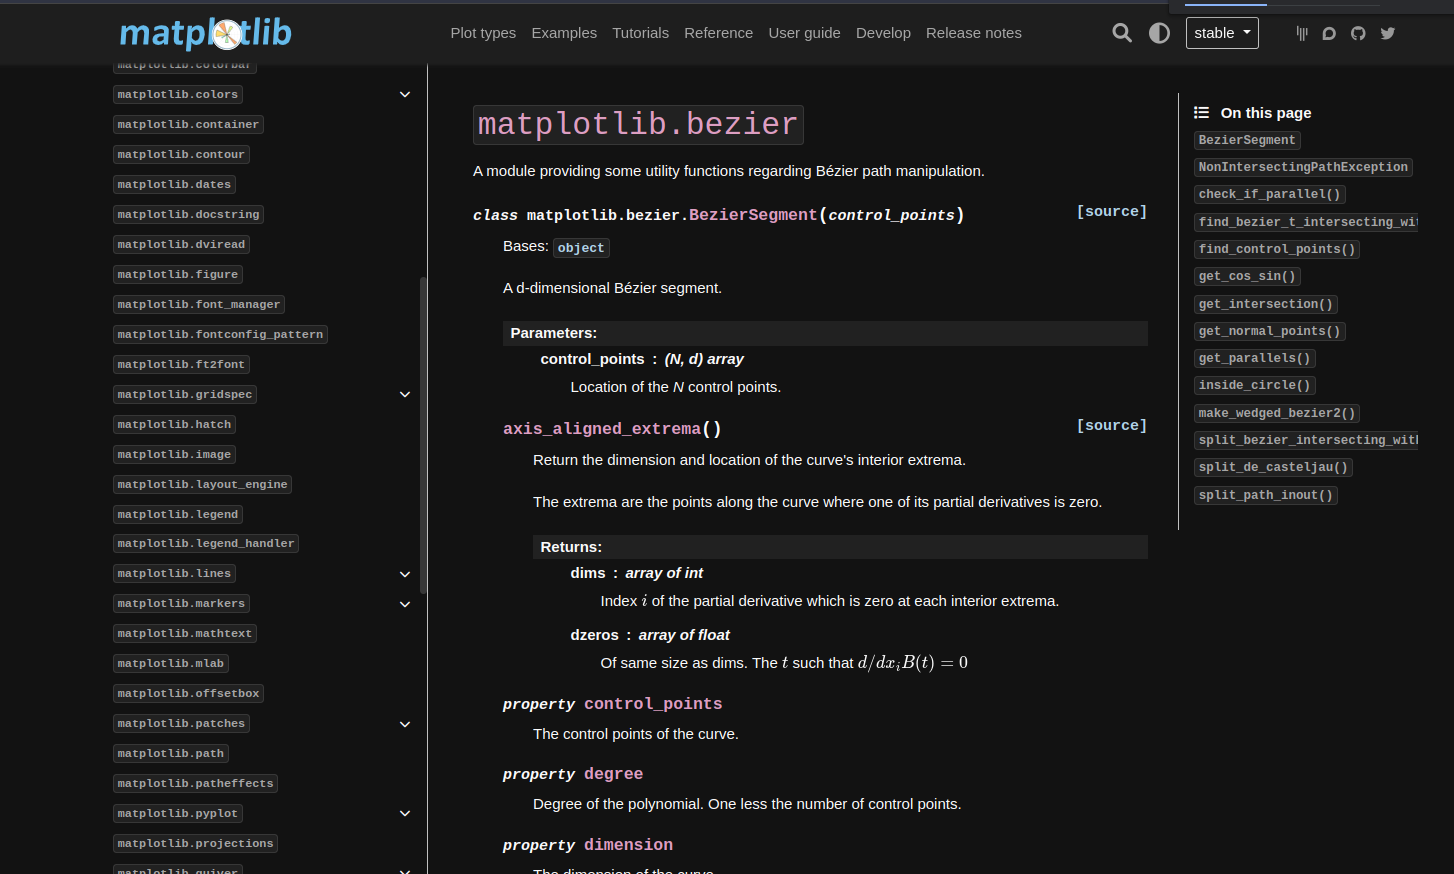
\includegraphics[width = 0.9 \linewidth]{bezier_code4.png}}
        \only<4>{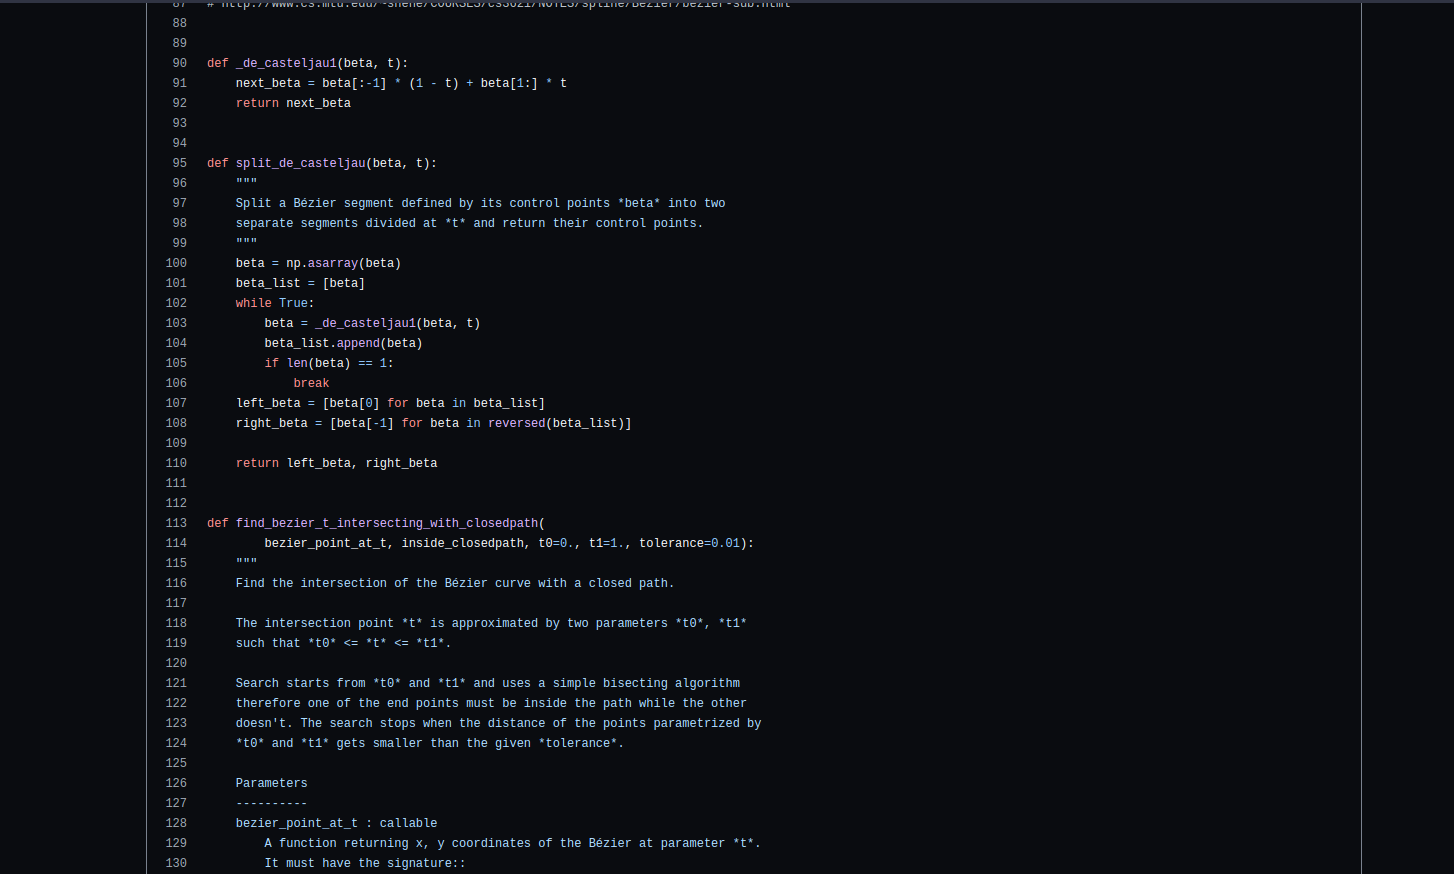
\includegraphics[width = 0.9 \linewidth]{bezier_code5.png}}
    \end{center}}
    \only<5>{E até mesmo montar a curva apenas com comandos python e biblioteca matplotlib
    \begin{center}
        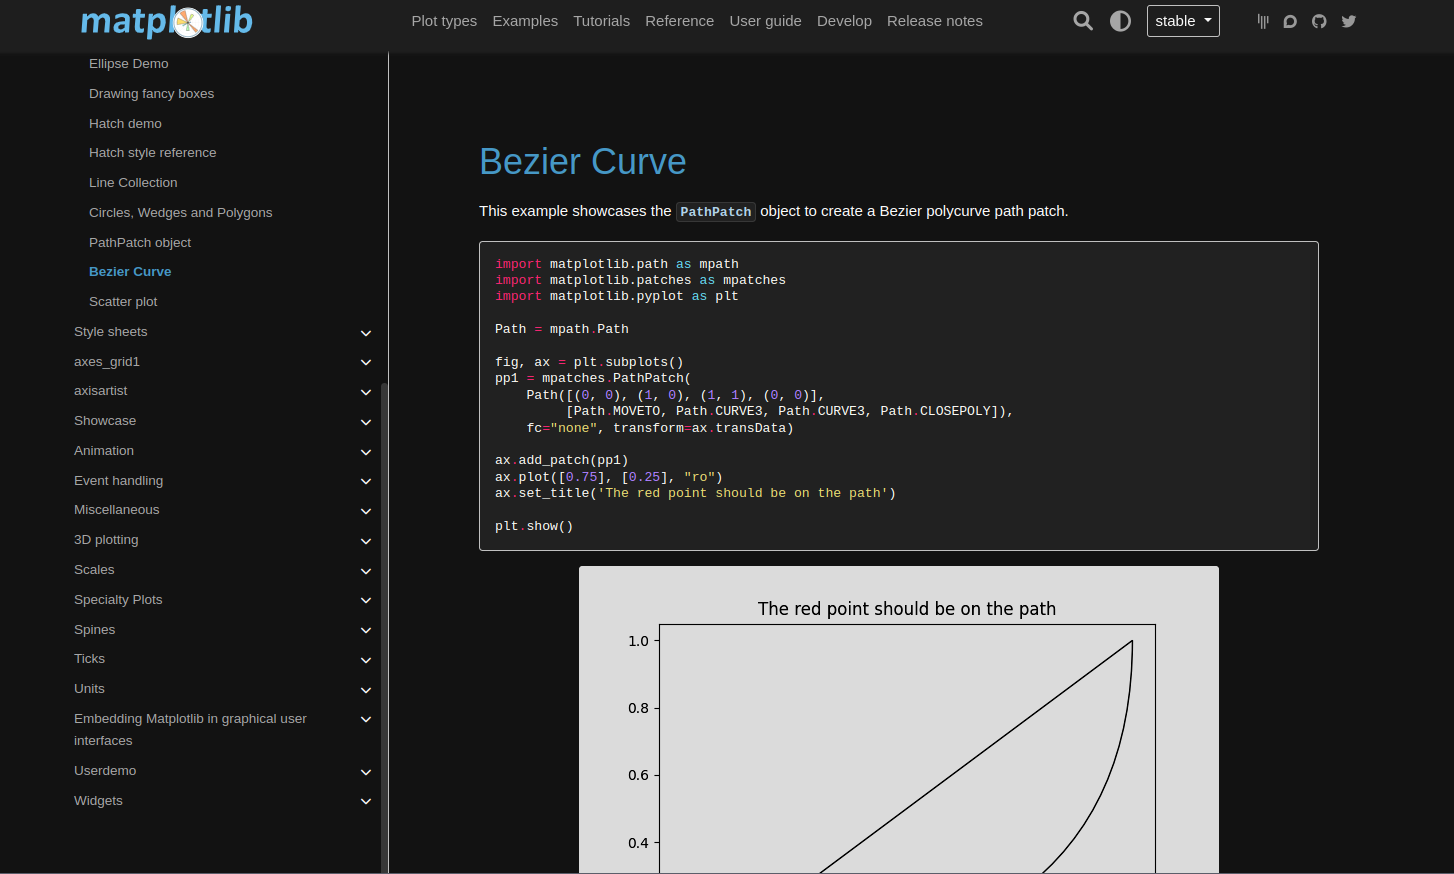
\includegraphics[width = 0.9 \linewidth]{bezier_code3.png}
    \end{center}
    }
\end{frame}

\subsubsection{Código}
\begin{frame}{Ideia}
    \only<1>{Como conversado em aula, a construção do código foi organiza-lo de maneira separada. A partir de uma construção. Dessa maneira:}\begin{enumerate}
        \item<1-5> \only<1-5>{Foi criado uma janela de pontos com o matplotlib;
        \begin{center}
            \only<3>{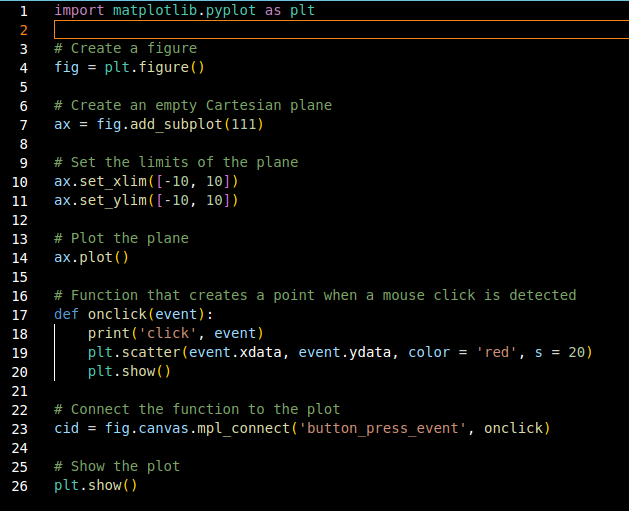
\includegraphics[width = 0.75 \linewidth]{construcao.png}}
            \only<4>{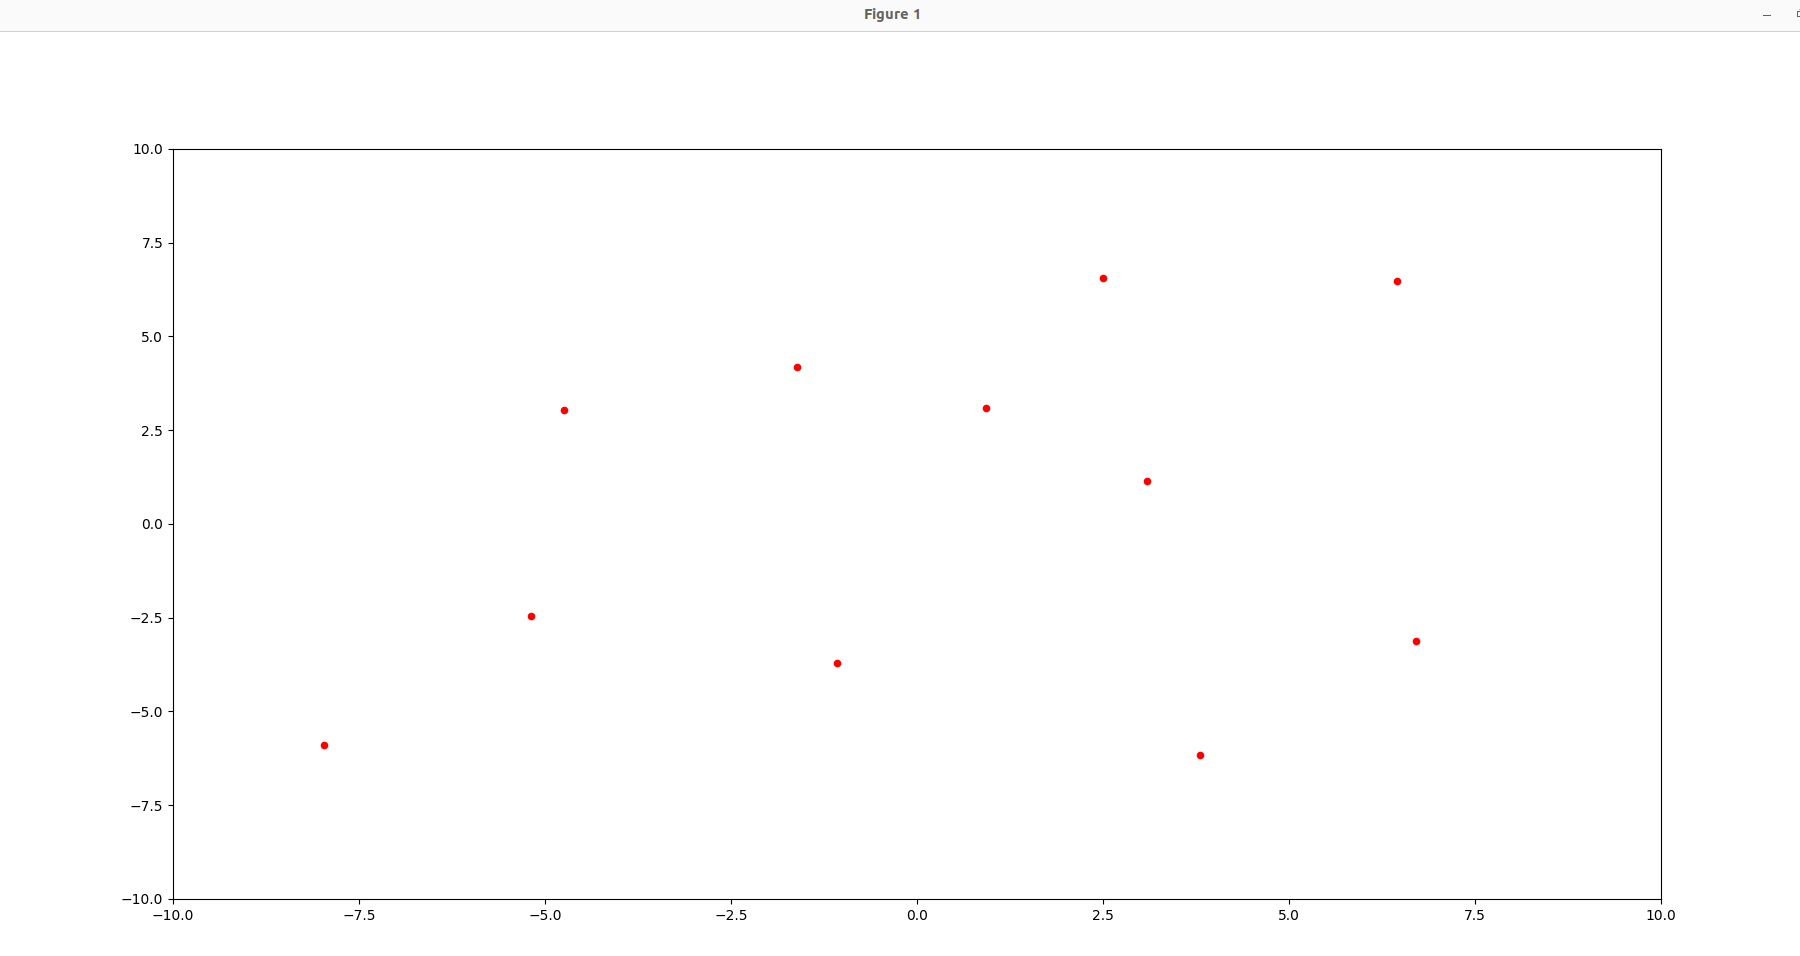
\includegraphics[width = 1 \linewidth]{construcao0.png}}
        \end{center}
        }
        \only<5>{Arquivo encontrado na pasta examples, arquivo examples3.py}
        \item<6-9> \only<6-9>{Em seguida, a janela foi ajustada para receber entradas de pontos. E com isso, com os pontos criados, cria-se segmentos. Portanto, cria-se um polígono de controle.
        \begin{center}
            \only<7>{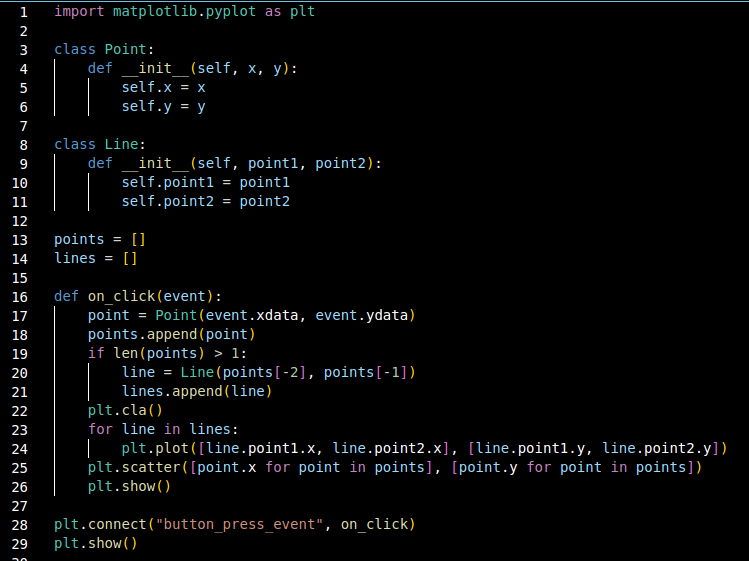
\includegraphics[width = 0.65 \linewidth]{construcao1.png}}
            \only<8>{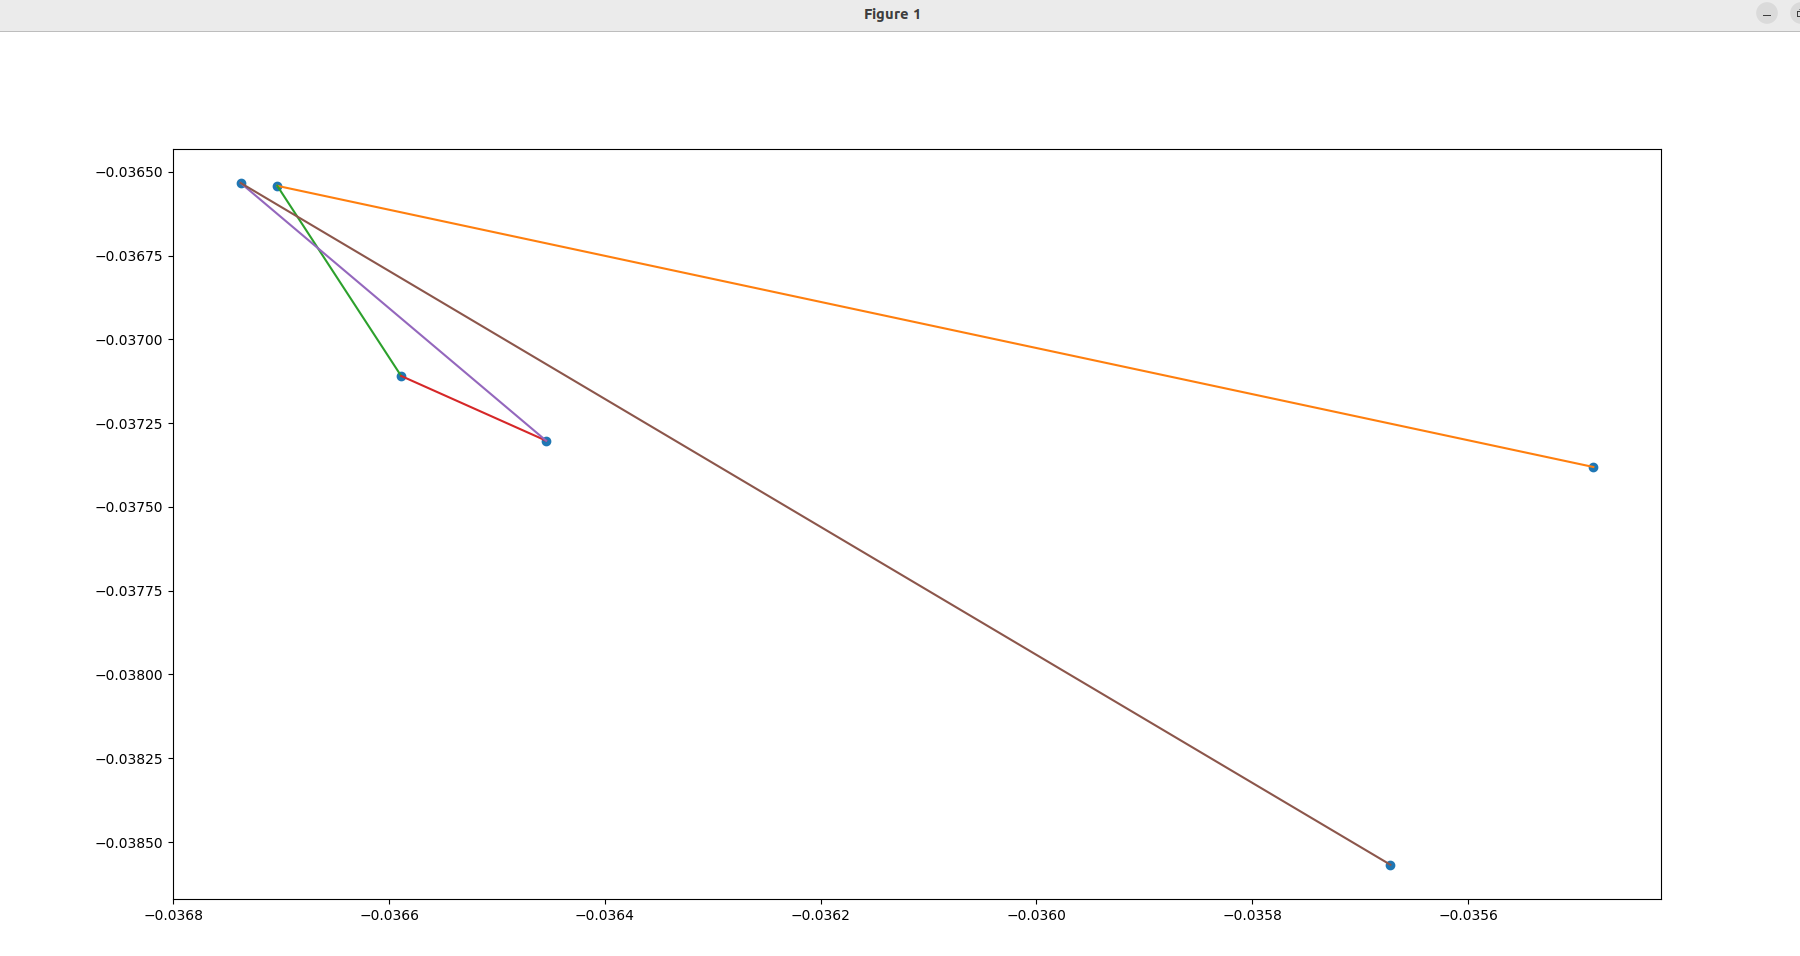
\includegraphics[width = 1 \linewidth]{construcao2.png}}
        \end{center}
        }
        \only<9>{Arquivo encontrada na pasta examples, arquivo example8.py}
        \item<10-15> \only<10-13>{Agora, é necessário trabalhar um pouco com a definição da curva de bézier. Para isto, olhemos a definição a partir da imagem. 
        \begin{minipage}{4cm}
        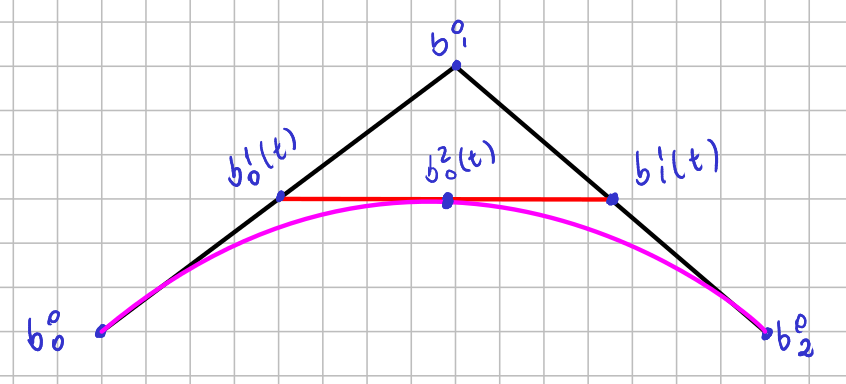
\includegraphics[width = 0.9 \linewidth]{construcao3.png}
        \end{minipage}\hfill
        \begin{minipage}{6cm} \\
        \only<11-13>{\begin{eqnarray} b_0^1(t) &=& (1-t)b_0^0 + tb_1^0 \\
                                    b_1^1(t) &=& (1-t)b_1^0 + tb_2^0
                            \end{eqnarray}
                            \only<12,13>{\begin{eqnarray}
                                b_0^2(t) &=& (1-t)b_0^1(t) + tb_1^1(t) \nonumber \Rightarrow \\
                                \only<13>{b_0^2(t) &=& (1-t)^2b_0^0 + 2t(1-t)b_1^0 + t^2b_2^0}\nonumber
                            \end{eqnarray}}}
        \end{minipage}
        }
        \only<14>{Para o cálculo de $b_0^n(t)$, $n = 3$. Ou seja, curva de bézier de grau 3. Temos
        \begin{center}
            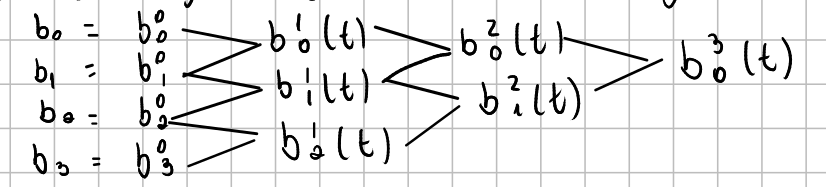
\includegraphics[width = 1 \linewidth]{construcao4.png}
        \end{center}
        }
        \only<15>{
        Portanto, o algoritmo que cria o polígono de construção deve realizar os mesmos processos, ou algo parecido com os cálculos. Assim, foi construído um algoritmo que depende da entrada t e os pontos dados.
        }
    \end{enumerate}
\end{frame}
\subsubsection{Polígono de controle com os pontos no parâmetro $t$}
\begin{frame}
    \only<1>{\begin{center}
            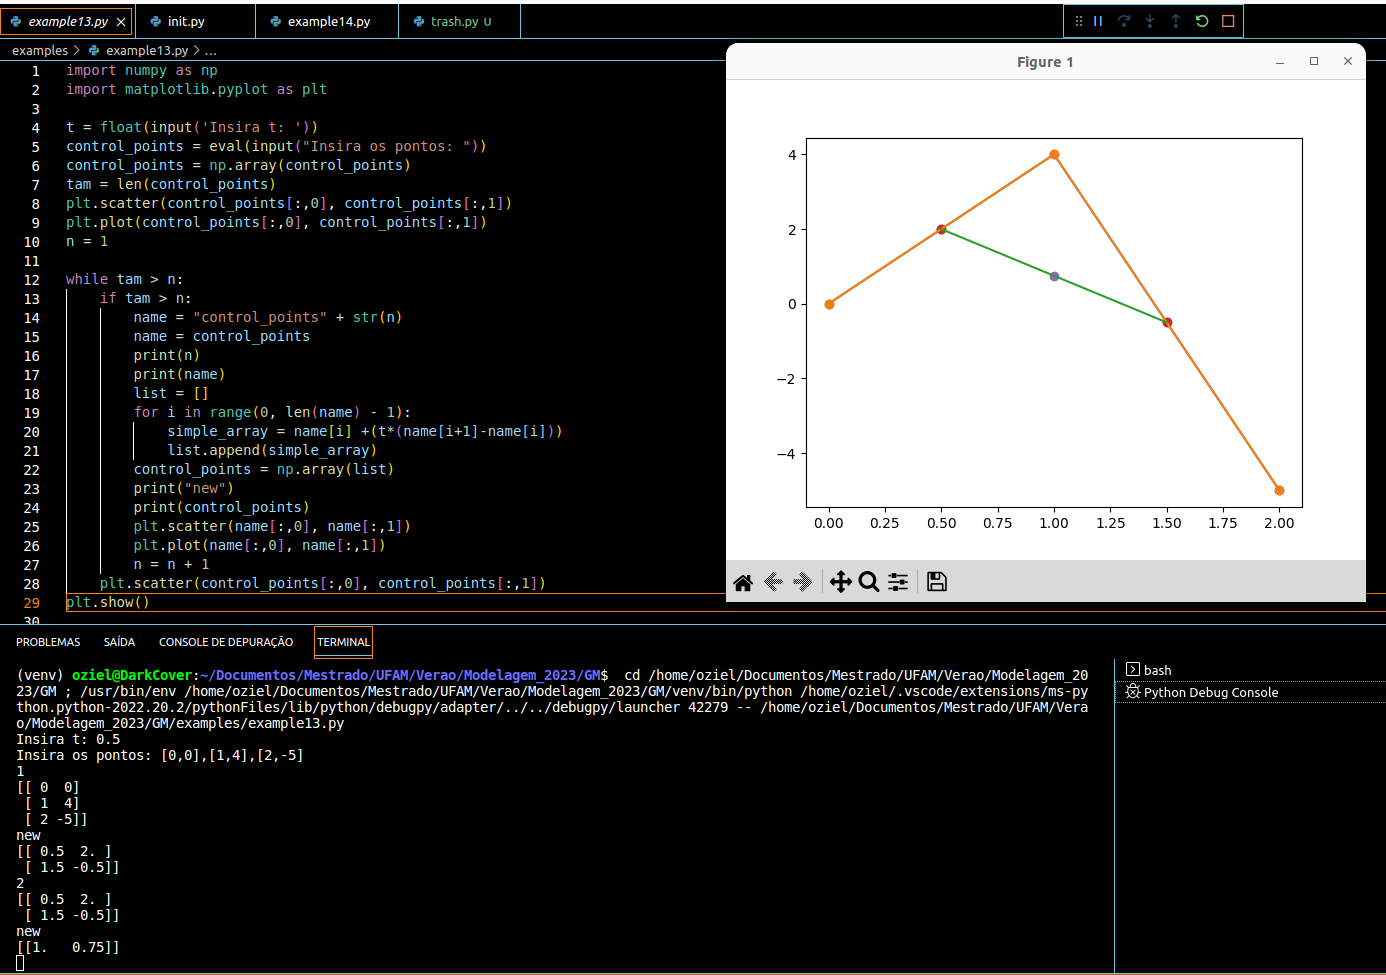
\includegraphics[width = 1 \linewidth]{construcao5.png}
    \end{center}}
    \only<2>{Este código pode ser encontrado na pasta example, arquivo example13.py}
\end{frame}

\subsubsection{Curva de Bézier}
\begin{frame}
    \only<1>{Para elaborar a curva de bézier, basta pega o último algoritmo criado e realizar o cálculo dos pontos com o t variando de 0 a 1. Nesse exemplo, foram criados 50 valores de t.}
    \only<2>{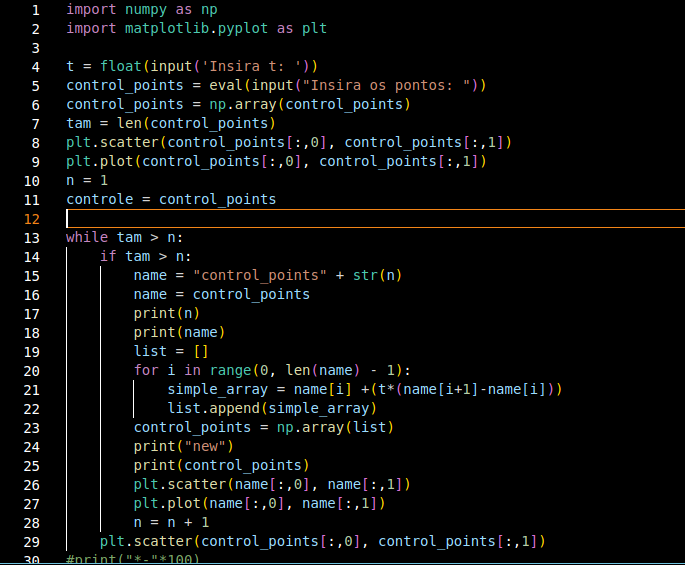
\includegraphics[width = 1 \linewidth]{construcao6.png}}
    \only<3>{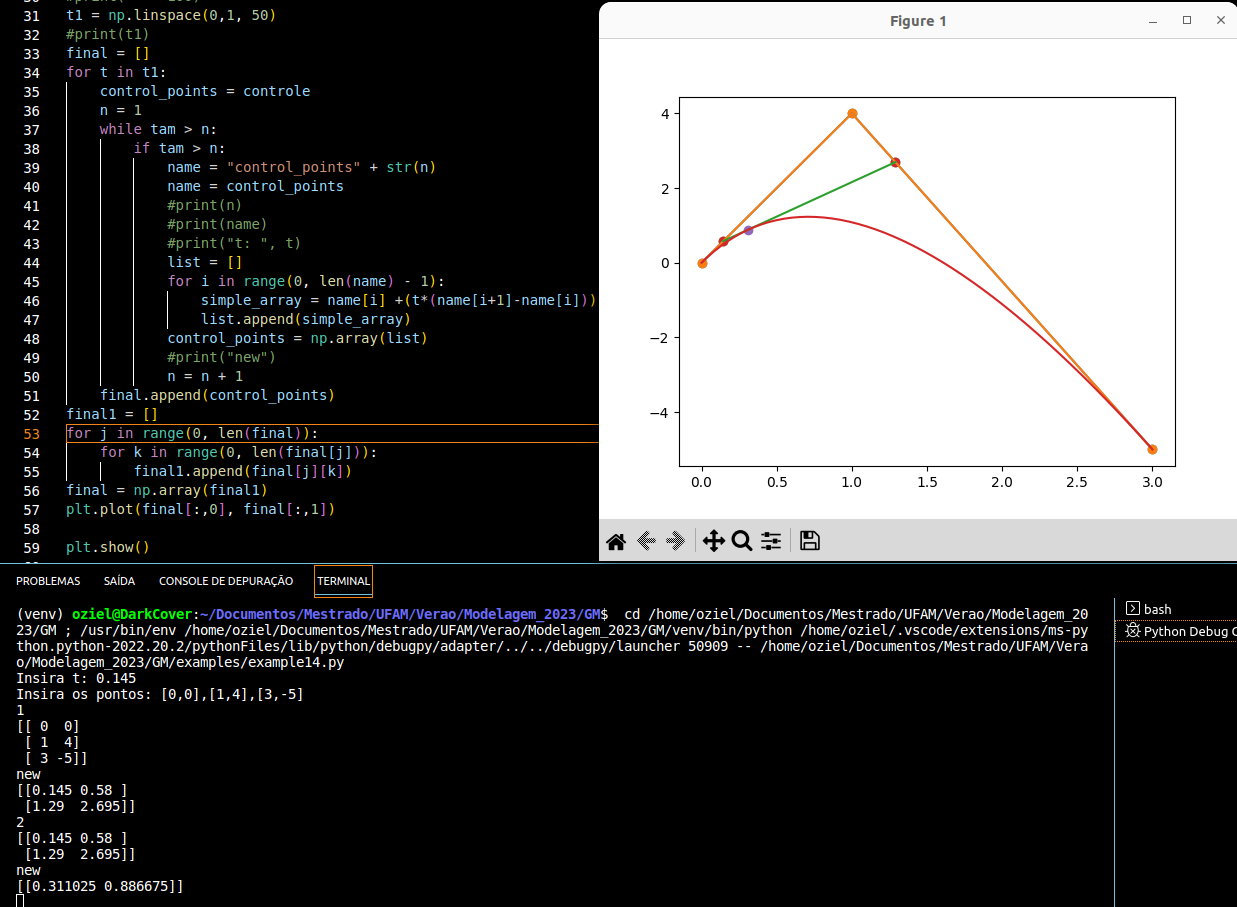
\includegraphics[width = 1 \linewidth]{construcao7.png}}
\end{frame}

\section{Classe Final}
\begin{frame}{Classe Final}
    Portanto, o trabalho final consiste na junção de todos os códigos citados em um único arquivo .py. Foi elaborado um arquivo classep.py que consiste no projeto final e pode ser encontrado na pasta  python$\_$project, arquivo classep.py. No perfil \hyperlink{https://github.com/oziieljuniior/GM}{Projeto da Curva}.
\end{frame}


\section{Referências}
\subsection{Links}
\begin{frame}{Links}
    \begin{itemize}
        \item \hyperlink{https://github.com/oziieljuniior/GM}{Projeto da Curva}
        \item \hyperlink{https://github.com/matplotlib/matplotlib/blob/v3.6.3/lib/matplotlib/bezier.py#L181-L305}{Código da documentação da Curva de Bézier do Matplotlib} 
        \item \hyperlink{https://matplotlib.org/stable/api/bezier_api.html#module-matplotlib.bezier}{Documentação da Curva de Bézier do Matplolib}
        \item \hyperlink{https://matplotlib.org/stable/gallery/shapes_and_collections/quad_bezier.html}{Exemplo de Curva de Bézier com matplotlib}
        \item \hyperlink{https://github.com/torresjrjr/Bezier.py}{Biblioteca da Curva de Bézier}
        \item \hyperlink{https://github.com/izabelacborges/cg-curves-python}{Exercício da Curva de Bézier}
        
    \end{itemize}
    
\end{frame}
\end{document}